\documentclass[aspectratio=169]{beamer}
\usetheme{Boadilla}

% ---------------------------------------------------------
% Premium Academic Color Theme (Slate Blue & Crimson Accents)
% ---------------------------------------------------------
\definecolor{navyblue}{RGB}{20, 54, 95}
\definecolor{crimsonred}{RGB}{141, 8, 28}
\definecolor{charcoal}{RGB}{43, 43, 43}
\definecolor{lightgray}{RGB}{245, 245, 245}

\usecolortheme[named=navyblue]{structure}
\setbeamercolor{title}{bg=navyblue, fg=white}
\setbeamercolor{frametitle}{bg=navyblue, fg=white}
\setbeamercolor{block title}{bg=navyblue, fg=white}
\setbeamercolor{block body}{bg=lightgray, fg=charcoal}
\setbeamercolor{block title alerted}{bg=crimsonred, fg=white}
\setbeamercolor{block body alerted}{bg=lightgray, fg=charcoal}

\setbeamertemplate{navigation symbols}{} % Hide default navigation icons
\setbeamertemplate{headline}{}

% Packages
\usepackage[utf8]{inputenc}
\usepackage{graphicx}
\usepackage{booktabs}
\usepackage{amsmath}
\usepackage{amssymb}
\usepackage{listings}
\usepackage{hyperref}

% Code snippet styles
\lstset{
    language=Python,
    basicstyle=\ttfamily\tiny,
    keywordstyle=\color{navyblue}\bfseries,
    commentstyle=\color{gray}\itshape,
    stringstyle=\color{crimsonred},
    showstringspaces=false,
    breaklines=true,
    backgroundcolor=\color{lightgray},
    frame=single,
    rulecolor=\color{lightgray}
}

% ---------------------------------------------------------
% Presentation Details
% ---------------------------------------------------------
\title[AMPT Course — Day 2]{Day 2: Relativistic Kinematics I \& II: Rapidity \& Pseudorapidity in Detail}
\subtitle{14-Day Hands-on Course on Heavy-Ion Phenomenology}
\author[MSc-Lecture Series]{Lecture}
\institute[HEP Group]{NIT-J, HEP-119}
\date{June 2026}

\begin{document}

% Slide 1: Title Slide
\begin{frame}
    \titlepage
\end{frame}

% Slide 2: 14-Day Course Syllabus Overview
\begin{frame}{Syllabus: 14-Day Hands-on Course Layout}
    \begin{columns}
        \begin{column}{0.5\textwidth}
            \footnotesize
            \textbf{Part I: Relativistic Kinematics}
            \begin{itemize}
                \item Day 1: Foundations of Relativistic Kinematics \& Experimental HEP
                \item \textbf{Day 2: Kinematics I \& II: Rapidity \& Pseudorapidity in Detail}
                \item Day 3: Kinematics III: Invariant Yield \& Phase Space Jacobian
                \item Day 4: Kinematics IV: Coordinate Calculator implementations
            \end{itemize}
            \vspace{0.05cm}
            \textbf{Part II: AMPT Physics \& Mechanics}
            \begin{itemize}
                \item Day 5: AMPT Evolution: HIJING, ZPC, Hadronization, ART
                \item Day 6: AMPT Data format: event headers \& parsing
                \item Day 7: Single-Particle Observables: Multiplicity \& $p_T$
            \end{itemize}
        \end{column}
        \begin{column}{0.5\textwidth}
            \footnotesize
            \textbf{Part III: Thermodynamics \& Collectivity}
            \begin{itemize}
                \item Day 8: Transverse Spectra, Identified Particles \& $m_T$ Scaling
                \item Day 9: Centrality \& Geometry: Glauber vs AMPT
                \item Day 10: Collective Flow: Elliptic Flow ($v_2$)
                \item Day 11: Medium Modification: ZPC Knobs \& Mean Free Path
            \end{itemize}
            \vspace{0.1cm}
            \textbf{Part IV: Advanced Scans \& Pipeline}
            \begin{itemize}
                \item Day 12: Energy Scan: Beam Energy Scan (STAR at RHIC)
                \item Day 13: Advanced Analysis
                \item Day 14: Wrap-Up: Reproducible HEP Data Pipeline
            \end{itemize}
        \end{column}
    \end{columns}
\end{frame}

\section{Pseudorapidity mapping}

% Slide 3: Polar Angle to Pseudorapidity mapping
\begin{frame}{Polar Angle to Pseudorapidity Mapping}
    \begin{block}{Theoretical Definition (Sahoo Eq. 5.138)}
        \small
        At ultra-relativistic limits ($p \gg m_0$), the momentum rapidity $y$ simplifies to a purely angular, geometric quantity called **Pseudorapidity** ($\eta$):
        \[ \eta = -\ln \tan \left( \frac{\theta}{2} \right) \]
        Where $\theta$ is the polar angle relative to the beam axis ($z$).
    \end{block}
    \begin{block}{Physical Advantages of Pseudorapidity}
        \footnotesize
        \begin{itemize}
            \item **No Particle ID (PID) needed:** Calculated solely from the emission angle $\theta$ of the trajectory in the tracker.
            \item **No magnetic field needed:** Does not require momentum information (only spatial tracking lines).
            \item **Symmetric / Odd behavior:** It is odd about $\theta = 90^\circ$ ($\eta=0$). That is, $\eta(180^\circ - \theta) = -\eta(\theta)$, reflecting forward-backward symmetry.
        \end{itemize}
    \end{block}
\end{frame}

% Slide 4: Table of Pseudorapidity vs Polar Angle
\begin{frame}{Angular Detector Mapping: $\theta$ vs. $\eta$}
    \begin{columns}
        \begin{column}{0.48\textwidth}
            \begin{block}{Angle to $\eta$ Reference (Sahoo Table 5.3)}
                \tiny
                \begin{tabular}{lcr}
                    \toprule
                    \textbf{Polar Angle $\theta$} & \textbf{Pseudorapidity $\eta$} & \textbf{Detector Region} \\
                    \midrule
                    $0^\circ$ & $\infty$ & Forward Beam pipe \\
                    $10^\circ$ & $2.44$ & Endcap region \\
                    $30^\circ$ & $1.32$ & Forward transition \\
                    $45^\circ$ & $0.88$ & Diagonal transition \\
                    $90^\circ$ & $0.00$ & Central Barrel \\
                    $135^\circ$ & $-0.88$ & Diagonal transition \\
                    $170^\circ$ & $-2.44$ & Backward transition \\
                    $180^\circ$ & $-\infty$ & Backward Beam pipe \\
                    \bottomrule
                \end{tabular}
            \end{block}
        \end{column}
        \begin{column}{0.52\textwidth}
            \begin{block}{Physical Trajectories (Sahoo Fig. 5.13)}
                \footnotesize
                \begin{itemize}
                    \item $\theta = 90^\circ$ ($\eta=0$): Particles fly straight out transversely.
                    \item $\theta \to 0^\circ$ ($\eta \to \infty$): Particles fly forward along the beam pipe.
                    \item High $|\eta|$ values denote regions extremely close to the beam line (demanding high spatial resolution trackers).
                \end{itemize}
            \end{block}
            \begin{alertblock}{Interactive Physics Simulator}
                Open in your browser:
                \begin{itemize}
                    \item \texttt{animations/05\_pseudorapidity\_detector\_angle.html} \quad {\tiny (Interactive polar angle $\theta$ vs. pseudorapidity $\eta$ detector mapping)}
                \end{itemize}
            \end{alertblock}
        \end{column}
    \end{columns}
\end{frame}

\section{Relativistic Transformations}

% Slide 5: Coordinate Changes of Variables
\begin{frame}{Coordinate Transformation: From $(y, p_T)$ to $(\eta, p_T)$}
    \begin{block}{Vector Decompositions (Sahoo Eq. 5.141 - 5.143)}
        \small
        By defining the pseudorapidity $\eta$ in terms of longitudinal momentum $p_z$ and total momentum magnitude $|\mathbf{p}|$:
        \[ e^\eta = \sqrt{\frac{|\mathbf{p}| + p_z}{|\mathbf{p}| - p_z}}, \quad e^{-\eta} = \sqrt{\frac{|\mathbf{p}| - p_z}{|\mathbf{p}| + p_z}} \]
        We can solve for the momentum component variables in terms of $(p_T, \eta)$:
        \[ |\mathbf{p}| = p_T \cosh \eta, \quad p_z = p_T \sinh \eta \]
        Which allows us to write the energy $E$ and transverse mass $m_T$ elegantly:
        \[ E = \sqrt{|\mathbf{p}|^2 + m_0^2} = \sqrt{p_T^2 \cosh^2 \eta + m_0^2} \]
    \end{block}
\end{frame}

% Slide 6: The Phase-Space Jacobian Factor
\begin{frame}{The Phase-Space Jacobian Transformation}
    \begin{block}{Rapidity to Pseudorapidity Mapping (Sahoo Eq. 5.147)}
        \small
        The distribution of particles as a function of pseudorapidity ($dN/d\eta$) is related to the rapidity distribution ($dN/dy$) via the phase-space Jacobian $J(y \to \eta) = \mathrm{d}y/\mathrm{d}\eta$:
        \[ \frac{\mathrm{d}N}{\mathrm{d}\eta \mathrm{d}p_T} = J(y \to \eta) \frac{\mathrm{d}N}{\mathrm{d}y \mathrm{d}p_T} = \sqrt{1 - \frac{m_0^2}{m_T^2 \cosh^2 y}} \frac{\mathrm{d}N}{\mathrm{d}y \mathrm{d}p_T} \]
        Where the Jacobian factor is exactly the particle's longitudinal velocity:
        \[ J(y \to \eta) = \frac{p}{E} = \beta \]
    \end{block}
    \begin{block}{Physical Consequence of Jacobian}
        \footnotesize
        \begin{itemize}
            \item **Massless limit ($m_0 \to 0$):** $J \to 1$, meaning $\mathrm{d}N/\mathrm{d}\eta \approx \mathrm{d}N/\mathrm{d}y$ (valid for photons or very high $p_T$ hadrons).
            \item **Massive limit ($m_0 > 0$):** $J < 1$ at mid-rapidity ($y \approx 0$). This creates a local, non-physical suppression in $\mathrm{d}N/\mathrm{d}\eta$ even if the underlying physical $\mathrm{d}N/\mathrm{d}y$ is flat.
        \end{itemize}
    \end{block}
\end{frame}

% Slide 7: AMPT Data Validation: dN/dy vs dN/deta
\begin{frame}{AMPT Data Validation: $\mathrm{d}N/\mathrm{d}y$ vs. $\mathrm{d}N/\mathrm{d}\eta$}
    \begin{columns}
        \begin{column}{0.5\textwidth}
            \begin{center}
                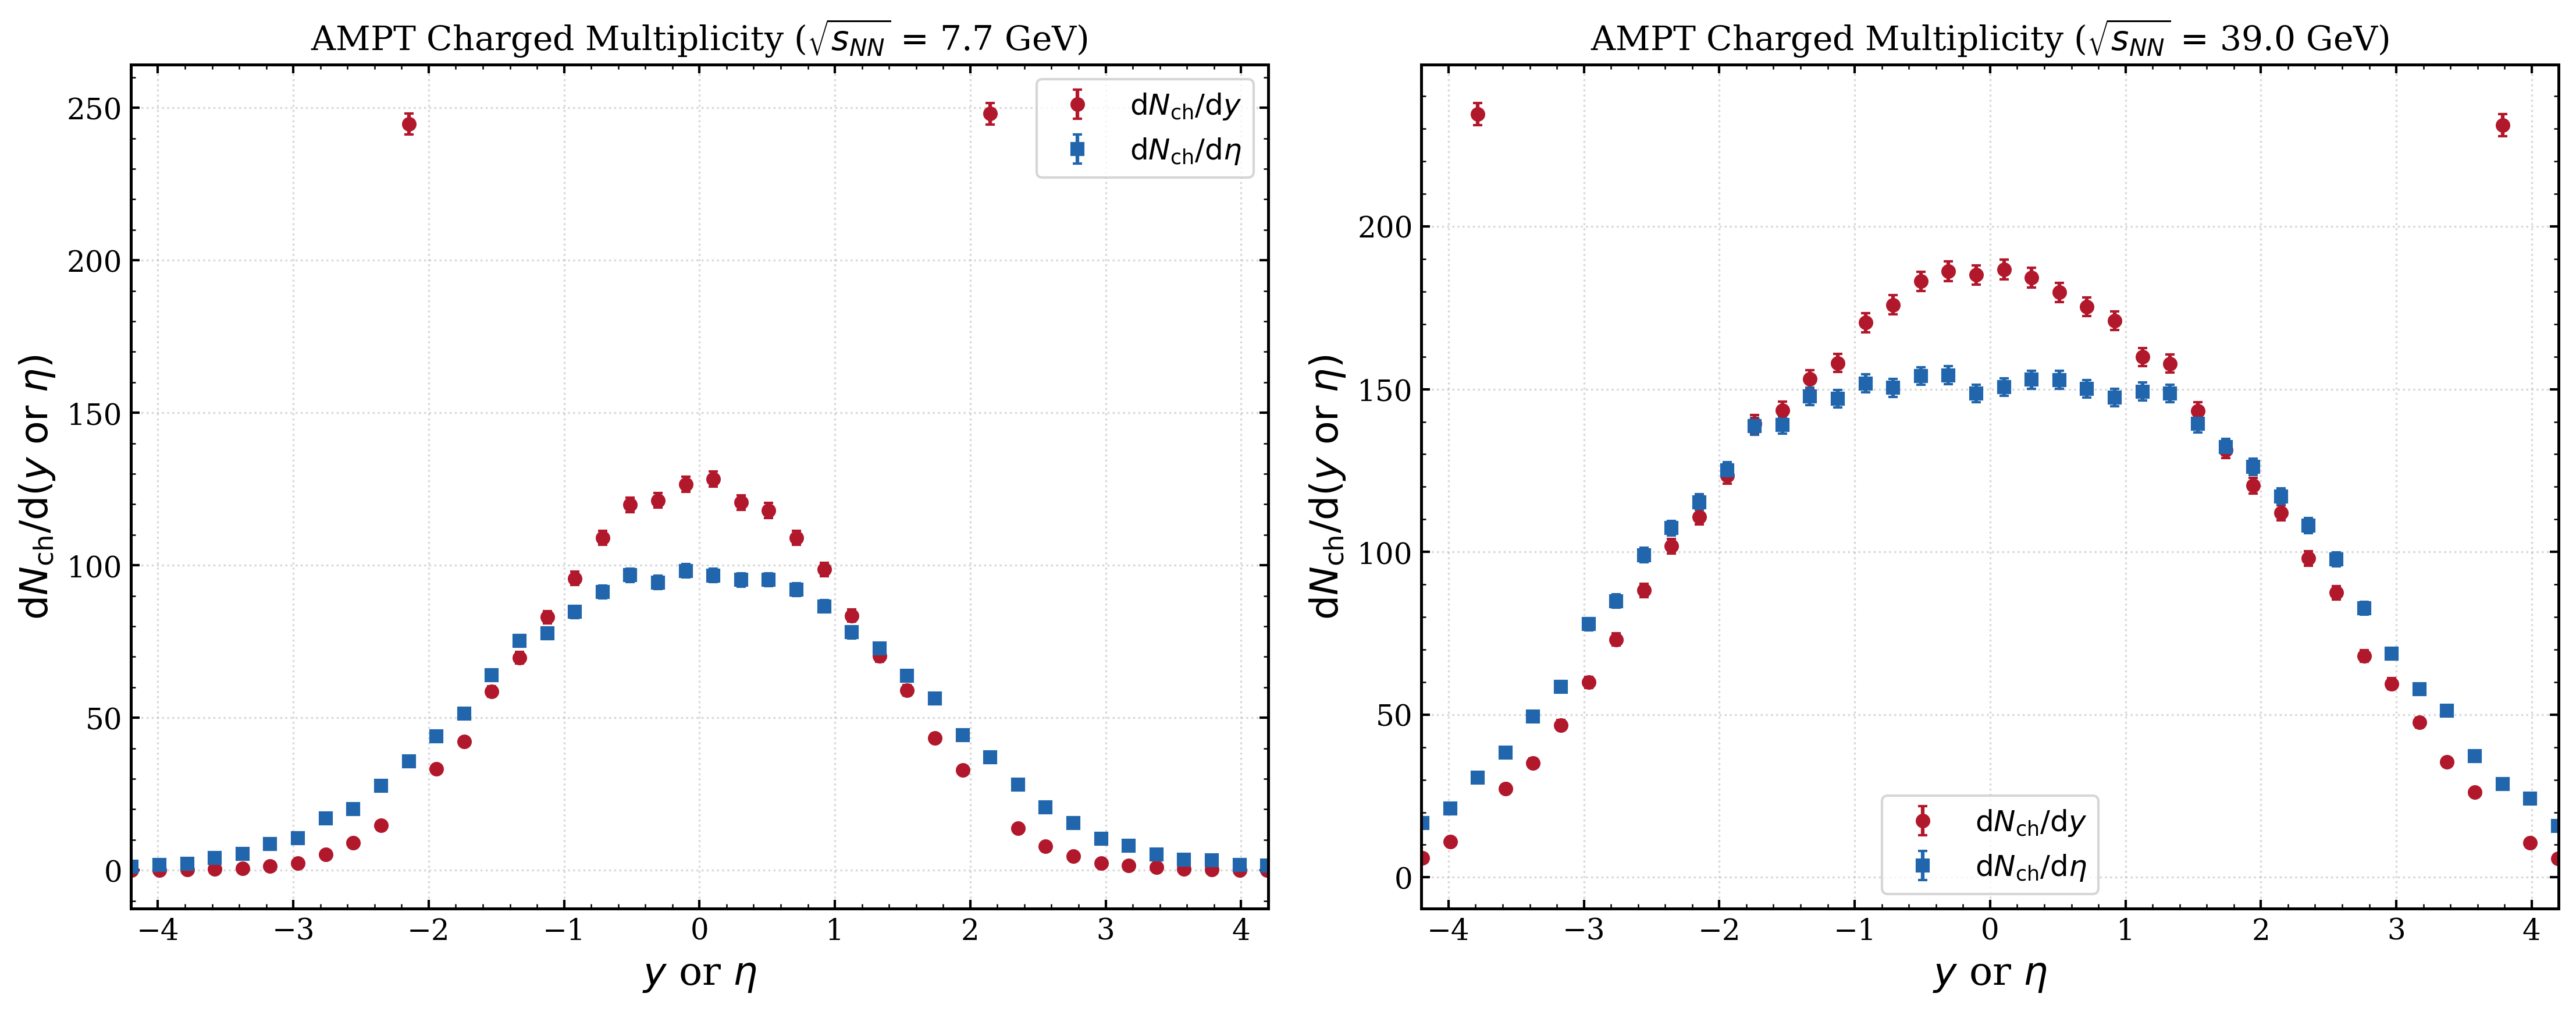
\includegraphics[height=0.62\textheight]{day2/day2_dndy_vs_dndeta.png}
            \end{center}
        \end{column}
        \begin{column}{0.5\textwidth}
            \footnotesize
            \begin{block}{Comparison of Yields (AMPT default)}
                \begin{itemize}
                    \item Plots show charged particle distributions in $\mathrm{Au}+\mathrm{Au}$ collisions at $\sqrt{s_{NN}} = 7.7$ and $39$ GeV.
                    \item **Rapidity ($\mathrm{d}N/\mathrm{d}y$)** exhibits a higher peak at mid-rapidity and drops off faster.
                    \item **Pseudorapidity ($\mathrm{d}N/\mathrm{d}\eta$)** is wider and has a slightly suppressed peak, caused directly by the integration over the Jacobian factor.
                \end{itemize}
            \end{block}
            \begin{alertblock}{Interactive Jacobian Explorer}
                Open in your browser:
                \begin{itemize}
                    \item \texttt{day2/day2\_rapidity\_jacobian\_explorer.html} \quad {\tiny (Interactive $p_T$, mass, and rapidity sweep dashboard)}
                \end{itemize}
            \end{alertblock}
        \end{column}
    \end{columns}
\end{frame}

% Slide 8: Mass-Dependent Mid-rapidity Dip
\begin{frame}{Mass-Dependent Mid-rapidity Dip in $\mathrm{d}N/\mathrm{d}\eta$}
    \begin{columns}
        \begin{column}{0.48\textwidth}
            \begin{center}
                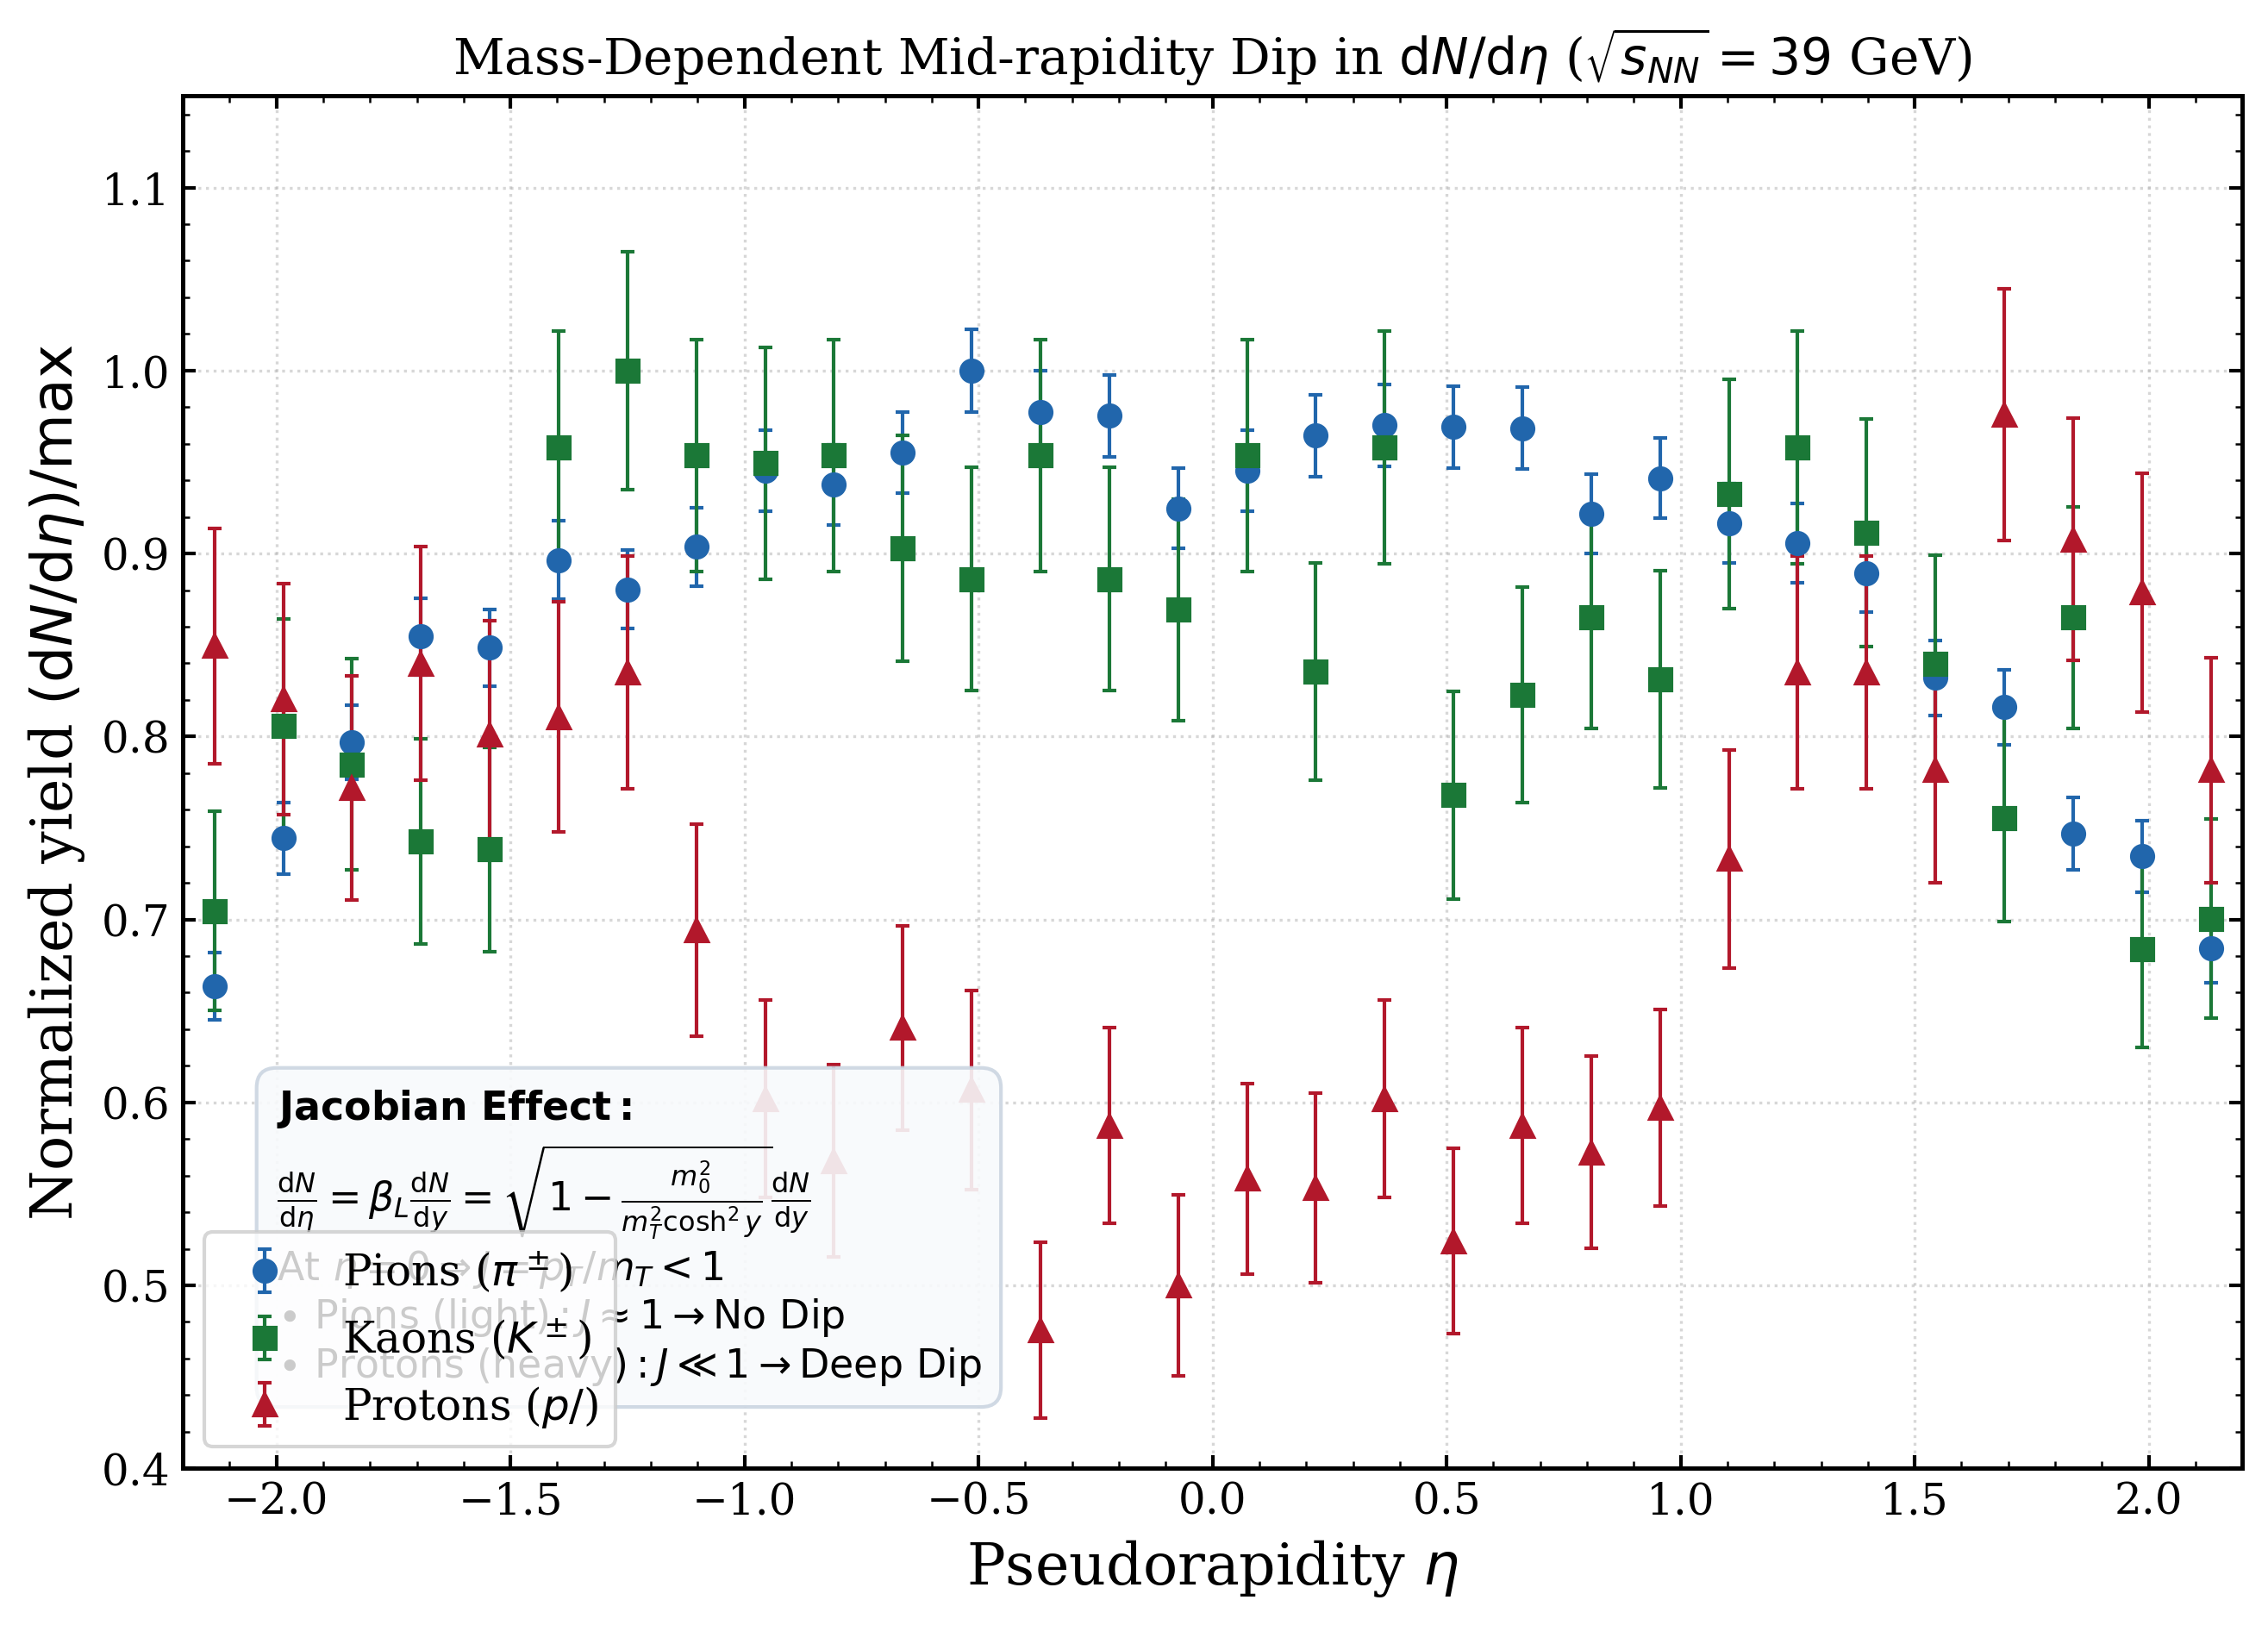
\includegraphics[height=0.65\textheight]{day2/day2_species_eta_dip.png}
            \end{center}
        \end{column}
        \begin{column}{0.52\textwidth}
            \footnotesize
            \begin{block}{Why do heavy particles dip at $\eta = 0$?}
                At mid-rapidity ($\eta = 0 \Rightarrow y = 0$), the Jacobian becomes:
                \[ J(0) = \frac{p_T}{m_T} = \frac{p_T}{\sqrt{p_T^2 + m_0^2}} \]
                \begin{itemize}
                    \item **Pions ($\pi^\pm$, $m_0 \approx 0.14$ GeV):** Light mass. $J(0) \approx 1$. No dip is visible in the yield.
                    \item **Kaons ($K^\pm$, $m_0 \approx 0.49$ GeV):** Medium mass. Shallow dip begins to emerge.
                    \item **Protons ($p/\bar{p}$, $m_0 \approx 0.94$ GeV):** Heavy mass. $J(0) \ll 1$ at low $p_T$, creating a deep, pronounced mid-rapidity dip.
                \end{itemize}
            \end{block}
            \begin{block}{Takeaway}
                This dip is purely a coordinate mapping artifact. The physics ($dN/dy$) remains flat or peak-like.
            \end{block}
        \end{column}
    \end{columns}
\end{frame}

\section{Hydrodynamics \& Speed of Sound}

% Slide 9: Landau Hydrodynamics & Rapidity Widths
\begin{frame}{Landau Hydrodynamics \& Rapidity Widths}
    \begin{block}{Landau Model Rapidity Distribution (Sahoo pg. 145-146)}
        \small
        In Landau's hydrodynamic model of relativistic expansion, the rapidity distribution of produced pions is described by a Gaussian:
        \[ \frac{\mathrm{d}N}{\mathrm{d}y} = \frac{N}{\sqrt{2\pi \sigma_y^2}} \exp \left( -\frac{y^2}{2\sigma_y^2} \right) \]
        Where the width of the rapidity distribution $\sigma_y$ relates to the center-of-mass energy and the speed of sound $c_s$ in the medium:
        \[ \sigma_y^2 = \frac{8}{3} \frac{c_s^2}{1 - c_s^4} \ln \left( \frac{\sqrt{s_{NN}}}{2 m_p} \right) \]
    \end{block}
    \begin{block}{Landau Model Scaling Limits}
        \footnotesize
        \begin{itemize}
            \item **Ideal Gas limit ($c_s^2 = 1/3$):** Prefactor becomes 1, so $\sigma_y = \sqrt{\ln(\sqrt{s_{NN}}/2m_p)}$.
            \item **Hadron Gas limit ($c_s^2 \approx 0.20$):** Premature freezing or lower speed of sound shrinks the rapidity width $\sigma_y$.
        \end{itemize}
    \end{block}
\end{frame}

% Slide 10: Speed of Sound & Phase Transition
\begin{frame}{Equation of State: Softest Point of QGP}
    \begin{columns}
        \begin{column}{0.48\textwidth}
            \begin{center}
                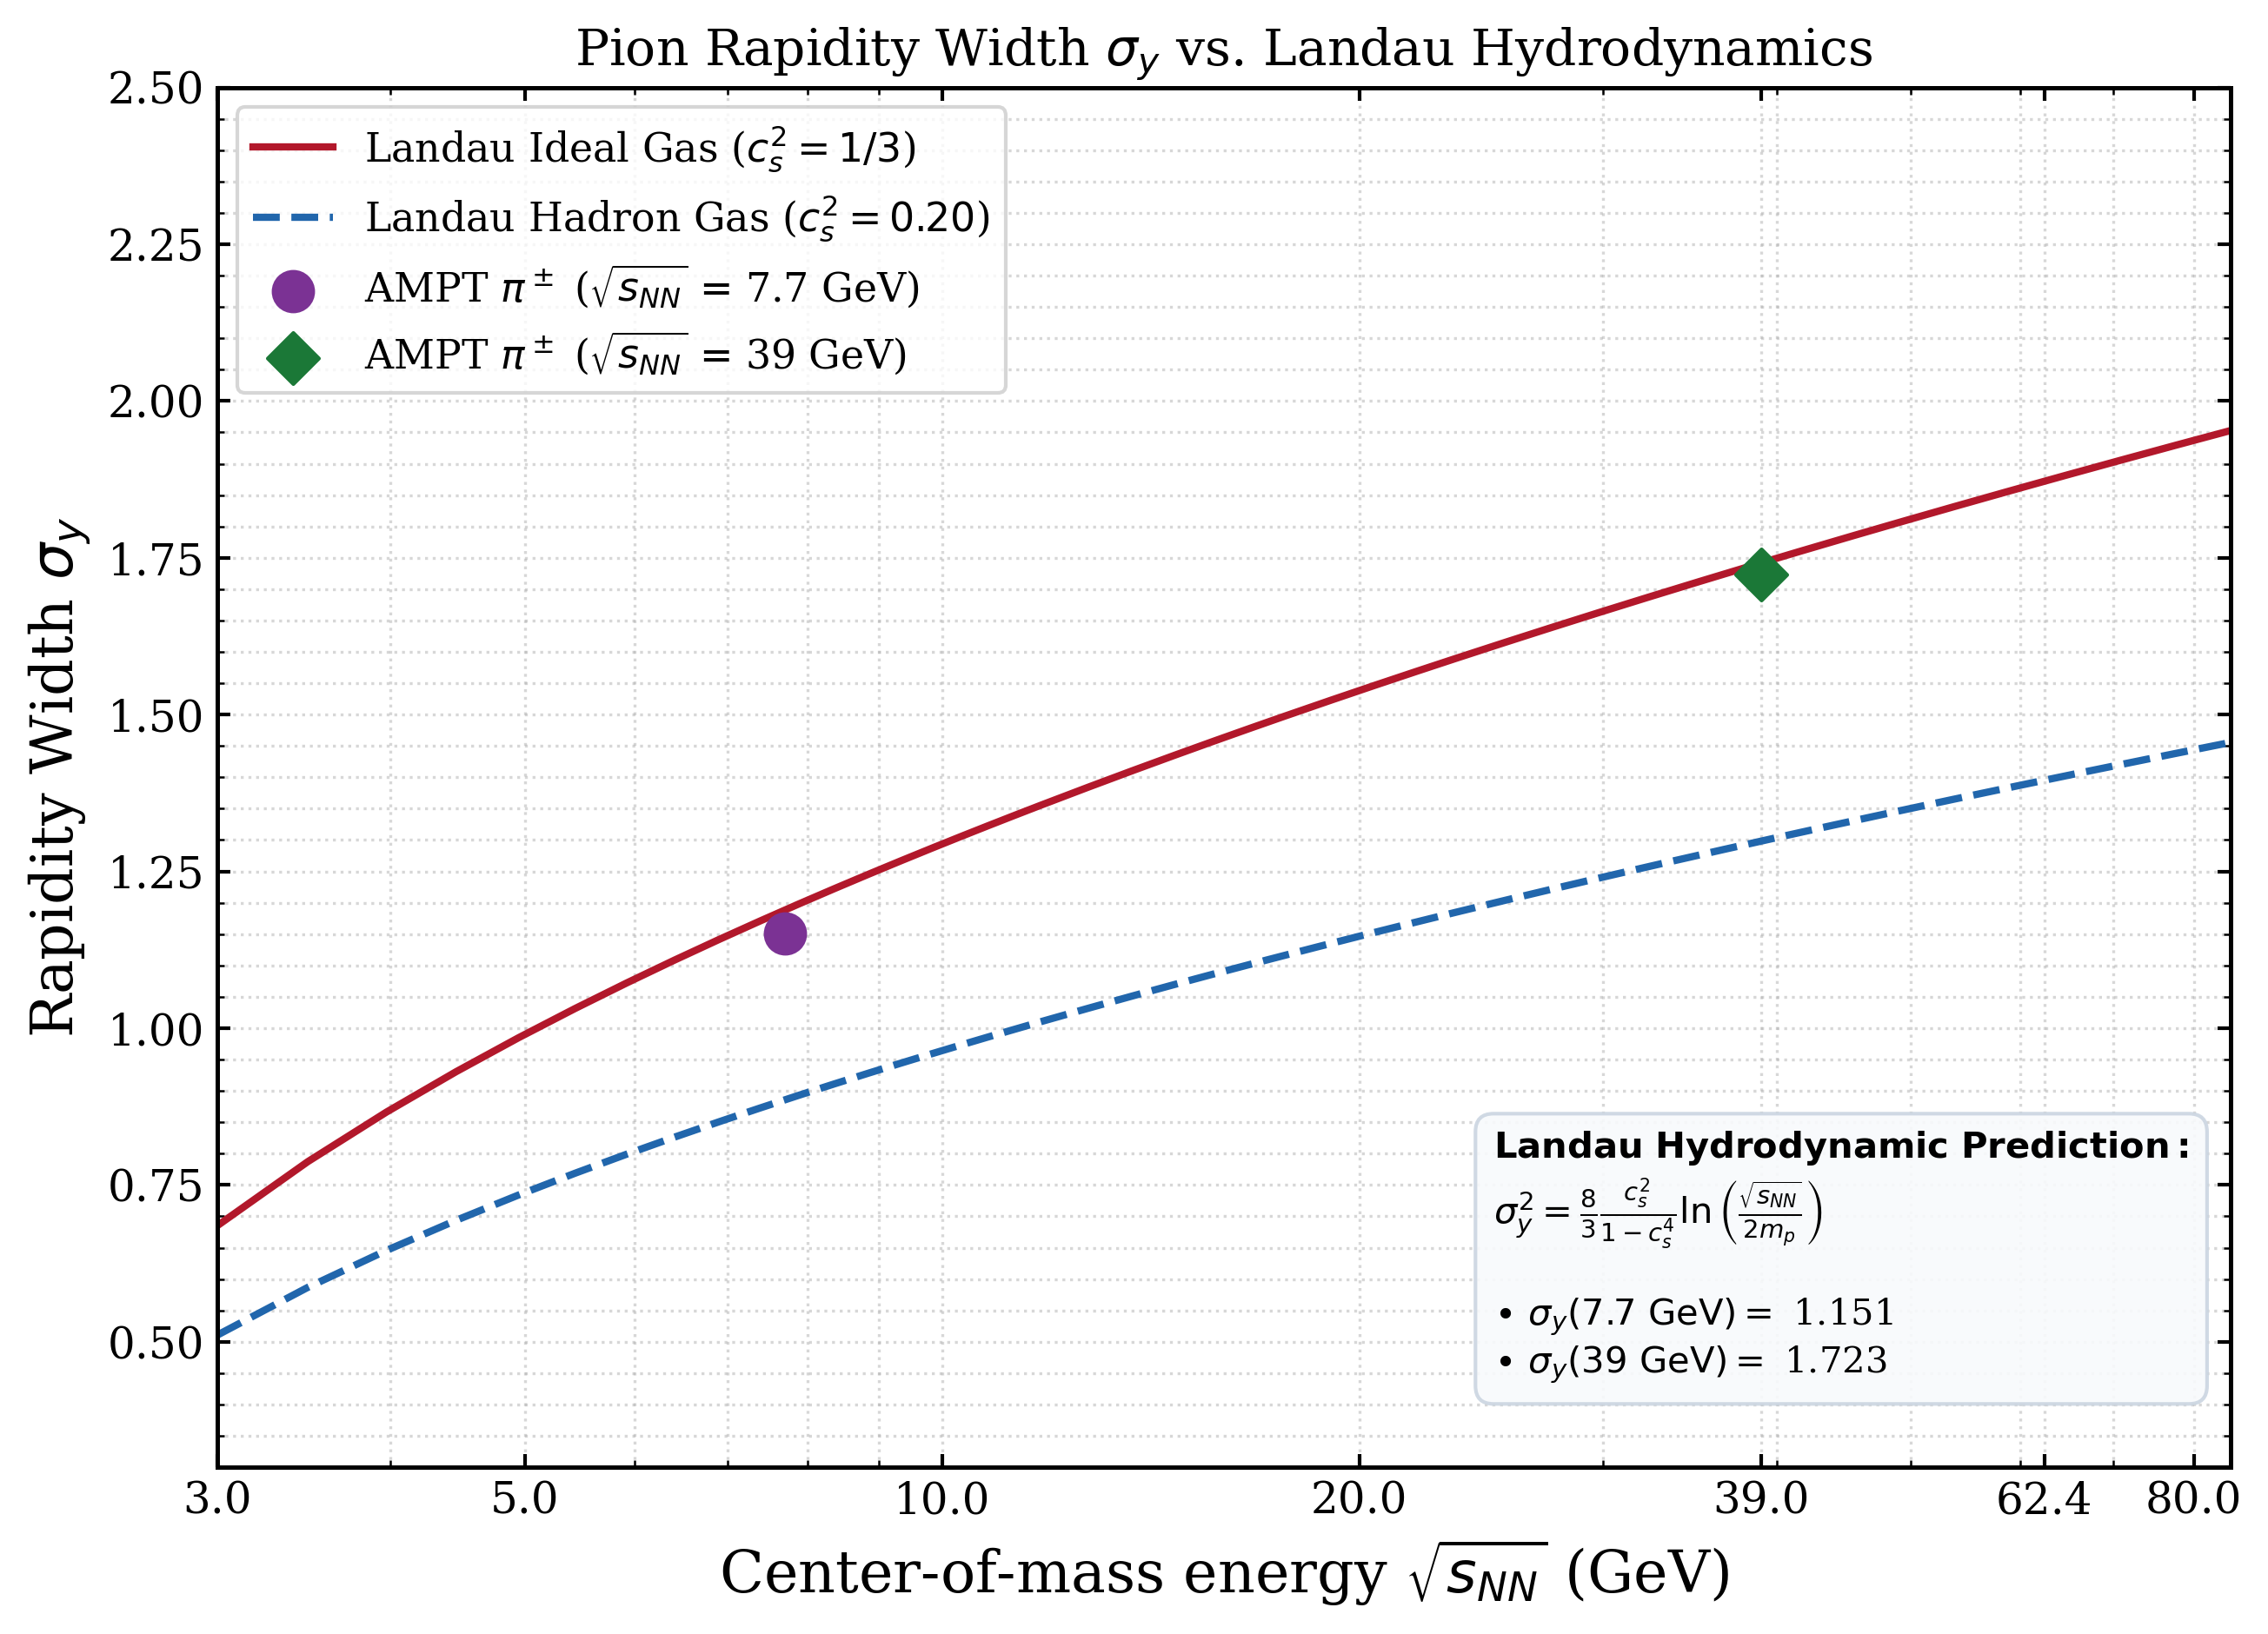
\includegraphics[height=0.65\textheight]{day2/day2_landau_width.png}
            \end{center}
        \end{column}
        \begin{column}{0.52\textwidth}
            \footnotesize
            \begin{block}{Speed of Sound $c_s^2$ Probe (Sahoo Fig. 5.16)}
                \begin{itemize}
                    \item By measuring the pion rapidity width $\sigma_y$ in AMPT and experiments, we can extract the effective speed of sound $c_s^2 = \partial P / \partial \epsilon$.
                    \item **The "Softest Point":** In heavy-ion energy scans, $c_s^2$ exhibits a minimum (a "dip") around $E_{\text{beam}} \approx 30$ AGeV ($\sqrt{s_{NN}} \approx 7.7$ GeV).
                    \item **Physics Interpretation:** This minimum denotes the softest point in the Equation of State (EoS), which is a classic signature of the transition from hadronic matter to QGP (crossover or first-order phase transition).
                \end{itemize}
            \end{block}
        \end{column}
    \end{columns}
\end{frame}

\section{Hands-On}

% Slide 11: Day 2 Hands-On Laboratory Exercises
\begin{frame}{Summary: Day 2 Hands-On Laboratory Exercises}
    \begin{block}{Objective: Analytical \& Data-Driven Rapidity Calculations}
        \small
        All exercises are framed in your Python files located in the \texttt{exercises/} and \texttt{day2/} folders:
    \end{block}
    \begin{enumerate}
        \footnotesize
        \item **Problem 1:** Calculate center-of-mass energy $\sqrt{s_{NN}}$ for RHIC Energy Scan values.
        \item **Problem 2:** Prove why collider configurations have a massive kinematic advantage over fixed-target configurations.
        \item **Problem 3:** Compute and verify Lorentz factors $\gamma$ and velocities $\beta$ for LHC Pb+Pb beams.
        \item **Problem 4:** Parse AMPT events, extract particle species (pions, kaons, protons), and plot the mass-dependent mid-rapidity dip in $\mathrm{d}N/\mathrm{d}\eta$.
        \item **Problem 5:** Extract the standard deviation (width $\sigma_y$) of pion rapidity and check compatibility with Landau's ideal gas limit vs. viscous gas models.
    \end{enumerate}
\end{frame}

\end{document}
